\documentclass[a4paper, 12pt]{article}
\usepackage[ruled, linesnumbered, noend]{algorithm2e}
\usepackage{setspace}
\usepackage{amsmath}
\usepackage[dvipsnames]{xcolor}
\usepackage{tikz}
\usepackage{verbatim}
\usepackage{amsthm}
\usepackage{wrapfig}
\usepackage{hyperref}
\usepackage{geometry}
\geometry{margin=1.125in}
\usepackage{mathtools}
\usepackage{breqn}
\usepackage{caption}
\usepackage{lipsum}
\usepackage{amssymb}
% \setlength{\parskip}{1 em}
\setlength{\parindent}{0 em}
\newcommand{\godel}{G\"{o}del }
\newcommand{\godels}{G\"{o}del's }
\theoremstyle{definition}
\newtheorem{definition}{Definition}
\captionsetup[figure]{name=\textit{Fig}}

\title{{\Large  \textit{On Hilbert, G\"{o}del, and the Quest for Formalization}}}
\author{M. Usaid Rehman}
\date{\today}

% TO DO: - remove whitespace near fig 1, image courtesy cantor 

\begin{document}
    \maketitle
    \setlength{\parskip}{0.75 em}
    % Introduction & idea of formalization 
    
    In 1931, an Austrian mathematician and logician named Kurt \godel performed an intellectual feat
    that would shock most mathematicians of the era -- bringing an abrupt end to the dreams of two generations of mathematics  
    while altering the course of mathematics itself in the process. \cite{ben-ari_mathematical_2012}

    Mathematicians of that time were on a quest to find a formal basis for all of mathematics -- a 
    set of axioms that were both consistent and complete. \godels incompleteness theorems were to bring an 
    end to this quest and change the way mathematicians thought about metamathematics. But before we look at \godel or 
    any of his ideas, let's zoom out and look at a slightly bigger picture. 

    \subsection*{The Axiomatic Method}
    Mathematicians often say that mathematics is based on the axiomatic method. But what do they exactly mean by that? 
    In the axiomatic method, we select a few basic facts or statements -- which we call \emph{axioms}. The axioms give us basic ideas 
    about the properties of the field of study and form the \textit{initial theory} about that field.
    You can think of axioms as the foundations of a building, upon which the rest of the structure will stand. 
    
    \begin{wrapfigure}{l}{0.35\textwidth}
        \centering
        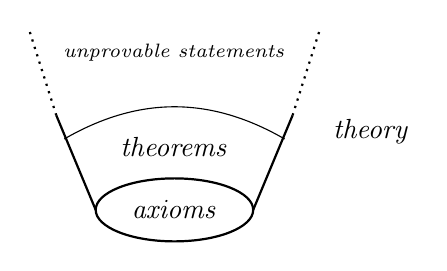
\begin{tikzpicture}
            \draw[thick] (0,0) ellipse (1cm and 0.4cm);
            \draw[thick] (-1,0) -- (-1.5,1.2);
            \draw[thick] (1,0) -- (1.5,1.2);
            \draw[thick, dotted] (1.5,1.2) -- (1.85, 2.3);
            \draw[thick, dotted] (-1.5,1.2) -- (-1.85, 2.3);
            \draw (1.4,0.9) to[out=150,in=30] (-1.4, 0.9);
            \node at (0,0) {\textit{axioms}};
            \node at (0,0.8) {\textit{theorems}};
            \node at (0,2) {\scriptsize \textit{unprovable statements}};
            \node at (2.5,1) {\textit{theory}};
        \end{tikzpicture}
        \caption{\textit{The structure of a  \\ theory.}}
        \vspace{-1 em}
        \label{theorystruct}
    \end{wrapfigure}
    Since mathematics makes use of the axiomatic method, we call it an axiomatic system. However our understanding of axioms has also changed 
    over the past two hundred years. Since the time of Euclid up till the 19\textsuperscript{th} century, axioms 
    had to be inherently meaningful -- in agreement with nature and the human experience. 
    
    However, advances in scientific thinking and 
    epistemology lead us to believe that experience and intuition could be misleading. This led to the concept of a 
    \textit{hypothetical} axiomatic system which allowed a lot more freedom over what axioms could be, since they no longer 
    had to obey the bounds of human experience and nature. 
  
    \subsection*{Crisis in Set Theory}
    
    The advent of hypothetical axiomatic systems gave rise to several different areas of mathematics, one of which was set theory. 
    Enter George Cantor -- an eccentric German mathematician who defined the concept of a set in 1895 as follows,
    \begin{definition}[Cantor's Set]
        A \textbf{set} is any collection of definite, distinguishable objects of our intuition or of our 
        intellect to be conceived as a whole (i.e., regarded as a singly unity).
    \end{definition}
    \vspace{-0.75 em}
    \begin{wrapfigure}{r}{0.3\textwidth}
        \vspace{-35pt}
        \centering 
        \includegraphics[scale=0.4]{cantor.jpeg}  
        \caption[Georg Cantor]{\textit{Georg Cantor}\footnotemark}
        \vspace{-10pt}
    \end{wrapfigure}
    \footnotetext{Image courtesy: \url{https://opc.mfo.de/detail?photo_id=10525}}
    In simpler terms, a set was a collection of mathematical objects. If an object $x$ belongs in a set $S$, we say 
    $x \in S$. If $x$ does not belong to $S$, then we say $x \notin S$. $x$ can either belongs in $S$ or it doesn't. There is no middle 
    ground.\footnote{This is called the \emph{Law of Excluded Middle}.} An analysis of Cantor's work revealed that he 
    used three principles to fashion his set theory. We call these principles the \textbf{Axioms of Extensionality}, \textbf{Abstraction} and \textbf{Choice}. 

    For simplicity's sake, we will not be taking a look at the formal definitions of these axioms. For a detailed 
    explanation see \cite{robic_foundations_2020}. Cantor's set theory quickly found several applications in various 
    mathematical areas. Sets were used to define ordered pairs, functions, and to construct the natural numbers by 
    Von Neumann. With his set theory, Cantor entered the wild world of infinities. 
    \vspace{-0.75 em}
    \subsubsection*{Logical Paradoxes}
    \vspace{-0.5 em}
    But with infinity, came problems. It had seemed like set theory could provide a simple and unified approach -- a foundation of all mathematics. 
    But in 1900, logical paradoxes were discovered in set theory -- unacceptable conclusions drawn from acceptable reasoning 
    from acceptable premises. These included the \textbf{Burali-Forti's Paradox}, \textbf{Cantor's Paradox} 
    and \textbf{Russell's Paradox}. 

    Russell's paradox is perhaps one of the most famous paradoxes in mathematics. Let's see what it's all about. 
    In 1901, using Cantor's set theory, Bertrand Russell found that you could have a set $\mathcal{R}$ that is both a member and 
    not a member of itself. Confusing, right? It should be -- it is a paradox after all. Russell defined $\mathcal{R}$ as \[
        \mathcal{R} = \{\mathcal{S} \hspace{0.25 em} | \hspace{0.25 em} \mathcal{S} \text{ is a set and $\mathcal{S}$ does not contain itself as a member}\}\]
    Due to the Law of Excluded Middle, $\mathcal{R} \in \mathcal{R}$ or $\mathcal{R} \notin \mathcal{R}$. But then using 
    the definition of $\mathcal{R}$, either of the two statements imply the other i.e., $\mathcal{R} \in \mathcal{R} \iff \mathcal{R} \notin \mathcal{R}$ -- which is 
    undoubtedly a paradox. 

    Why do we care about paradoxes? For starters, in theories which contain a logical statement where the statement is 
    both true and false, we can deduce any other statement of the theory. The reason for this is beyond the scope of this 
    essay and would require several months of study of logic and mathematics -- so we will conveniently ignore it. The point is 
    that such a theory would be useless since every statement in this theory would be true which is of no cognitive use to us. 

    \subsubsection*{Schools of Recovery}
    Paradoxes frightened mathematicians. They wanted a nice, clean system with no paradoxes. However, this was going to be an 
    incredibly difficult task. Three schools of mathematical thought emerged that contributed against the struggle against paradoxes. 
    These schools of thought had different approaches yet their end goal was the same -- find a unified basis for the mathematical system which is 
    free from paradoxes. 

    \begin{wrapfigure}{r}{0.3\textwidth}
        \centering
        \vspace{-1 em}
        \includegraphics[scale=0.15]{russell.jpg}
        \caption[russel]{\textit{Bertrand Russell}\footnotemark}
        \vspace{-1.75 em}
    \end{wrapfigure}
    \footnotetext{Image courtesy: \href{https://www.nationaalarchief.nl/onderzoeken/fotocollectie/a96fca82-d0b4-102d-bcf8-003048976d84}{https://www.nationaalarchief.nl/onderzoeken}}
    The first school was \textit{intuitionism}. Intuitionism argued for greater rigor in the process of mathematical proofs. 
    It was initiated by Jan Brouwer and further developed by Arend Heyting. In their view, mathematical proofs should be driven by the process of construction. This required 
    unprecedented rigor and caused a lot of mathematics to simply be tossed out the window. Intuitionism was not widely accepted since no one wanted to make such sacrifices. 

    Then we have \textit{logicism}. Logicism attempted to found mathematics based entirely on logic. Some proponents were 
    George Boole, Giuseppe Peano, Gottlob Frege -- each contributing in their own way to the puzzle at large.
    
    \begin{wrapfigure}{l}{0.3\textwidth}
        \centering 
        \includegraphics[scale=0.25]{Hilbert.jpg}
        \caption[hilbert]{\textit{David Hilbert}\footnotemark}
        \vspace{0 em}
    \end{wrapfigure}
    \footnotetext{Image courtesy: \url{https://commons.wikimedia.org/wiki/File:Hilbert.jpg}}
    Their goal was to create a language based on logic that could clearly express mathematical ideas without
    the ambiguity of a natural language. 
    
    Later proponents of logicism were Alfred Whitehead and the famous Bertrand Russell. To avoid his own paradox, 
    Russell came up with the \textit{Theory of Types} which would be the basis of Whitehead \& Russell's book \textit{Principia Mathematica}. 
    Principia Mathematica (\textit{PM}) managed to avoid all \emph{known} paradoxes and included long, cumbersome deductions of known results. However, 
    it was not known that the \textit{PM} avoided possibly unknown paradoxes as well or if all true statements were 
    provable within \textit{PM}. These problems were known as the \textit{Consistency Problem} of \textit{PM} and \textit{Completeness Problem} of \textit{PM} respectively. 
    
    The last school was \textit{formalism}. Spearheaded by David Hilbert -- a central figure in our story -- formalism wanted to retain 
    all classical mathematics while also establishing a unified basis for mathematics. Formalists had an entirely different approach. They wanted to focus on the 
    structure (syntax) instead of the meaning (semantics) of mathematical ideas. Therefore, 
    they worked on the formal-language formulation of mathematical activities. This is where our quest for formalization 
    officially starts. 

    \subsection*{Formalism}
    The first and perhaps most important step of this quest was attempting to define a formal axiomatic system. 
    The separation of syntax and semantics was the starting point. In order to manipulate mathematical ideas, 
    a metamathematical language was needed -- for which a formal axiomatic system formed the basis.
    \vspace{-0.75 em}
    \subsubsection*{Formal Axiomatic Systems}
    \vspace{-0.5 em}
    A formal axiomatic system offers:
    \vspace{-1 em}
    \begin{enumerate}
        \item a rigorously defined \textit{symbolic language};
        \vspace{-0.5 em}
        \item a set of \textit{rules of construction} -- syntactic rules used to build \textit{formulas} of the language;
        \vspace{-0.5 em}
        \item a set of \textit{rules of inference} -- rules used to build sequences of formulas, called \emph{derivations} or \emph{formal proofs}.
    \end{enumerate}

    A \textit{formula} is a sequence of symbols of the language and some formulas are distinguished as axioms. Given some formulas, 
    one can infer new formulas by applying rules of inference. Formulas that can be derived by 
    a finite sequence of inferences are called \textit{theorems}. Axioms, theorems and other formulas construct a \textit{theory} belonging to the 
    formal axiomatic system. 

    Since a theory developed within a formal axiomatic system is almost entirely syntactic, the only thing 
    that can be examined about it are its expressions, the syntactic properties of expressions and the relations between them.
    Because these are unambiguously determined by the formal system, the syntactic aspects of the theory can be analyzed without semantic issues. 
    Now, one can raise questions \textit{about the theory}. These questions; however, are not part of the theory itself 
    but instead form a \textit{metatheory} or a `theory about the theory'.

    \begin{figure}[h]
        \centering 
        \includegraphics[scale=0.3]{metatheory.png}
        \caption{A statement about the theory belongs to its metatheory.}
    \end{figure}

    Around the time these ideas were developed, the \textit{Consistency} and \textit{Completeness} Problem of \textit{PM} were
    gaining traction. Formalism gave mathematicians hope in answering such metamathematical questions. However, 
    the ultimate goals of formalism were even more ambitious. They intended to develop \emph{all} 
    mathematics in \textit{one} formal axiomatic system; and \textit{prove} that such mathematics is free of \textit{all} known and unknown paradoxes. 

    \subsubsection*{Formalization of Logic, Arithmetic and Set Theory}
    In order to develop any theory in a logically sound way, a formal axiomatic system must offer all the logical principles and tools. 
    Therefore, formalism collected the work of all the logicists in this regard and created a formal axiomatic system for logic 
    called \textit{First-Order Logic}, denoted by $\mathbf{L}$. This system contained basic rules of inference and 
    symbols that are used for proof writing today. 
    
    Other formal axiomatic systems are practically extensions of First-Order Logic. They contain whatever is in $\mathbf{L}$
    along with some additional axioms, symbols etc. Such as system is called a first-order formal axiomatic system and its theories are called first-order theories.
    One of these is the Formal Arithmetic $\mathbf{A}$ which formalizes arithmetic of the natural numbers. Since the natural numbers $\mathbb{N}$ play 
    a central role in constructing other numbers, it was important to formalize their arithmetic. 

    \begin{figure}[h]
        \centering 
        \begin{minipage}{0.45\textwidth}
            \centering 
            \includegraphics[width=0.5\textwidth]{Ernst_Zermelo_1900s.jpg}
            \caption[ernie]{\textit{Ernst Zermelo}\footnotemark}
        \end{minipage}
        \begin{minipage}{0.45\textwidth}
            \centering 
            \includegraphics[width=0.5\textwidth]{fraenkel.jpg}
            \caption[frankel]{\textit{Abraham Fraenkel}\footnotemark}
        \end{minipage}
    \end{figure}
    \footnotetext[5]{Image courtesy:
        \href{https://www.gettyimages.co.uk/detail/news-photo/portrait-of-the-german-mathematician-ernst-zermelo-1900s-news-photo/141551246}
        {
            \texttt{www.gettyimages.co.uk/detail/news-photo/zermelo}
        }
    }
    \footnotetext{Image courtesy: \url{https://commons.wikimedia.org/wiki/File:Adolf_Abraham_Halevi_Fraenkel.jpg}}
    Lastly, set theory had to be formalized as well. In Cantor's naive set theory, there were several paradoxes. Therefore, 
    mathematicians had to create a system where there were some restrictions on sets and their sizes. This difficult task was 
    undertaken by Ersnt Zermelo and Abraham Fraenkel over 1908--1930. They defined a formal axiomatic system \textbf{ZF} which 
    could derive all important theorems of Cantor's set theory while avoiding all \textit{known} logical paradoxes. This has become 
    the standard set theory now. When Cantor's axiom of choice is added to this theory, it is called $\mathbf{ZFC}$. 
    
    We will not be looking at the axioms of these theories for the sake of brevity and simplicity, but the more mathematically-inclined reader 
    is encouraged to explore the axioms of these systems further. 

    \subsection*{Hilbert's Program}
    
    Till this point, the quest for formalization seems promising. David Hilbert wanted to use formal axiomatic systems to 
    axiomatize all of mathematics and eliminate all paradoxes. Therefore, he proposed what is called \textit{Hilbert's Program}.
    \vspace{-1 em}
    \subsubsection*{Foundational Problems of Mathematics}
    \vspace{-0.75 em}
    Before mathematicians could even begin to perform this task, they had to understand and answer four fundamental 
    problems in the foundation of mathematics - the consistency, completeness and decidability problems. 
    \vspace{-0.75 em}
    \begin{enumerate}
        \item \textit{Consistency Problem}. Let \textbf{F} be some first-order theory. Suppose if $F$ is a formula in \textbf{F} such that 
        both $F$ and $\neg F$ \footnote{$\neg$ is used to represent the negation of a statement.} can be derived in \textbf{F}. Then the 
        contradictory formula $F$ and $\neg F$, i.e. $F \land \neg F$ can be derived in \textbf{F}. Such a theory is 
        called inconsistent. In an inconsistent theory, all possible formulas can be derived as true -- which is of no use to us. 
        \vspace{-0.3 em}        
        \item \textit{Completeness Problem}. Let \textbf{F} be a consistent first-order theory. In this case, for a formula $F$, both $F$ and $\neg F$ 
        are not derivable. But what if neither $F$ nor $\neg F$ can be derived? Such a formula is said to be independent of the theory \textbf{F}. This is undesirable 
        since these means that our theory has ``holes''. Therefore, we want every formula to be either provable or refutable.    
        \vspace{-0.3 em}
        \item \textit{Decidability Problem}. This problem poses an interesting question. Let \textbf{F} be a consistent and complete 
        theory. Consider a formula $F$ of theory \textbf{F}. If we can't prove or refute $F$, that is simply due to our own 
        incapability and not because of the limitations of the theory itself. Suppose that some algorithm called a decision procedure 
        existed that would tell us -- in a finite amount of time -- if a formula can or cannot be proved in a theory \textbf{F}. This would mean 
        that the theory \textbf{F} is decidable.    
    \end{enumerate} 

    \subsubsection*{Hilbert's Goals}
    \vspace{-0.75 em}
    From 1920--28, Hilbert gradually formed a list of goals -- called Hilbert's program --- that should be attained to form a new basis 
    for mathematics without any paradoxes. These goals were:
    \vspace{-0.75 em}
    \begin{enumerate}
        \item[A.] find a formal axiomatic system \textbf{M} having a computable set of axioms and capable of proving all the theorems of mathematics;
        \vspace{-0.3 em} 
        \item[B.] prove that \textbf{M} is complete, i.e., there are no holes in the theory;
        \vspace{-0.3 em} 
        \item[C.] prove that \textbf{M} is consistent -- there are no contradictions and paradoxes;
        \vspace{-0.3 em} 
        \item[D.] construct an algorithm that is a decision procedure for \textbf{M}.     
    \end{enumerate}

    \subsubsection*{Decidability of \textbf{M}: \textit{Entscheidungsproblem}}
    \vspace{-0.75 em} 
    Mathematicians immediately set to work, investigating how they would attain these four goals. But there was a lot of work to be done. Firstly, what 
    would this axiomatic system \textbf{M} look like? It was agreed that it should contain First-Order Logic \textbf{L} and 
    Formal Arithmetic \textbf{A}. \cite{robic_foundations_2020}

    The fourth of Hilbert's goals, the \textit{Entscheidungsproblem} was very important. It aimed to construct an algorithm 
    \textit{D\textsubscript{Entsch}} which would decide whether a formula $F$ can be derived in \textbf{M}. 
    Finitism was at the heart of these mathematicians. A proof or derivation was to be constructed using a finite 
    number of steps using a finite number of axiomatic rules. The algorithm looked roughly like this:
    \begin{algorithm}
        Systematically generate finite sequences of symbols of \textbf{M} \\
        \ForEach{\upshape newly generated sequence}{
            \If{\upshape sequence is a proof of $F$ in \textbf{M}}{answer \textsc{yes} and halt}
            \Else{
                \If{\upshape sequence is a proof of $\neg F$ in \textbf{M}}{answer \textsc{no} and halt}
            }
        }
        \caption{\textit{D\textsubscript{Entsch}}}
    \end{algorithm}

    If we assume that we can either prove or refute $F$, the procedure will always halt. Around the time this problem was proposed,
    there was general consensus that \textbf{M} would be complete. The decidability question was intrinsically related to the completeness 
    and consistency questions. If \textbf{M} were consistent, then at most one of $F$ and $\neg F$ could be proven. In addition, if \textbf{M} were complete as well 
    then at least one of $F$ or $\neg F$ can be proven. Therefore, in this case a decision procedure would exist, and \textbf{M} would be 
    decidable. \cite{zach_hilberts_2019}

    This boils down to a simple implication:
    \vspace{-0.5 em}
    \begin{figure}[h]
        \centering
        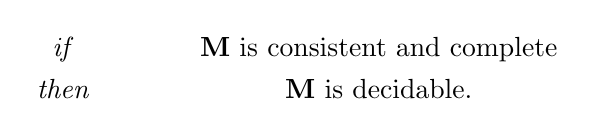
\begin{tikzpicture}
            \node at (0,0) {\textit{if}};
            \node at (4,0) {\textbf{M} is consistent and complete};
            \node at (0,-0.5) {\textit{then}};
            \node at (4,-0.5) {\textbf{M} is decidable.};
        \end{tikzpicture}
        \vspace{-0.5 em} 
    \end{figure} 
    
    Progress, right? At this point of the story it seems like the mathematicians' jobs have been laid out in front of them 
    in a simple way. Most of the mathematicians of the time got their hopes up -- perhaps the end was in sight.
    
    \newpage
    \subsection*{The Incompleteness Theorems}
    
    At this point in our story, enters an eccentric young Austrian-American mathematician -- Kurt G\"{o}del. Not only was \godel a mathematician, he was 
    also a logician and analytic philosopher. Alongside other mathematicians, he too was busy working on 
    Hilbert's mission.
    
    \begin{wrapfigure}{r}{0.3\textwidth}
        \centering
        \vspace{-2 em}
        \includegraphics[scale=0.4]{godel2.jpeg}
        \caption[godel]{\textit{Kurt \godel}\footnotemark}
    \end{wrapfigure}
    \footnotetext{Image courtesy: \url{https://www.ias.edu/scholars/godel}}
    Although, no one expected that he would be the cause of the demise of Hilbert's mission.
    This demise came in the form of \godels Incompleteness Theorems -- two theorems that proved the incompleteness 
    of mathematics using mathematics.\cite{raatikainen_2020}
    He was only twenty-five years old when he came up with his theorems -- an undoubtedly extraordinary feat.
    He proved two theorems which were to alter the course of mathematics and by extension, computer science forever. 
    He proved that: 
    \vspace{-0.5 em}
    \begin{center}
        \texttt{G\"{O}DEL'S INCOMPLETENESS THEOREMS} \\
        \texttt{For any consistent formal axiomatic system that expresses basic facts about arithmetic:
        } \vspace{-1 em}
        \begin{itemize}
            \item[\texttt{1.}] \texttt{There are true statements that are unprovable within the system.}
            \vspace{-0.3 em}
            \item[\texttt{2.}] \texttt{The system's consistency cannot be proven within the system.}  
        \end{itemize}
    \end{center}
    \vspace{-0.5 em}
    The first theorem states that any formal axiomatic system cannot prove every possible truth about the theory. This means that 
    there are ``holes'' in the system and our system is not complete. The second theorem says that if we have a set of axioms 
    we cannot use the same axioms to prove their own consistency. How G\"{o}del proved these theorems is an interesting topic -- but not 
    what this essay is going to be about.\footnote{\href{https://www.quantamagazine.org/how-godels-incompleteness-theorems-work-20200714/}
    {See this essay for a detailed look at the theorems and their proofs.}}
   \vspace{-1 em}
    \subsubsection*{The Fate of Hilbert's Program}
    \vspace{-0.75 em}
    Each of \godels theorems were a heavy blow to Hilbert's program. How did \godels results relate to a foundational mathematics, or in other words, 
    to the formal axiomatic system \textbf{M}? When we stated the theorems, we were being slightly dishonest. The actual proofs 
    were done specifically for the formal arithmetic \textbf{A} and then later generalized to other formal axiomatic systems. 
    A generalization of the Second Incompleteness Theorem states that if a consistent theory \textbf{F} contains \textbf{A}, then 
    \textbf{F} cannot prove its own consistency. This holds if \textbf{F} := \textbf{M} and therefore, a consistent basis for mathematics can't be found. 
    Such was the end of Hilbert's program. 

    However, Hilbert's program has had a lasting legacy. It helped provide a language to mathematicians to communicate ideas 
    with less ambiguity. Hilbert's decidability problem also lead to the birth of computability theory which became 
    one of the most studied areas in the coming decades. On a philosophical level, it shows that replacing human thought and reflection in mathematics is an illusion, 
    and that mathematics selfishly hides its truths -- only revealing these truths to 
    humans who demonstrate sufficient creativity, inspiration and ingenuity. 
    
    \godels genius ended the search for a consistent, complete formal axiomatic system for mathematics. It also led to 
    new forefronts in the philosophy of mathematics and even in popular philosophy -- becoming a common fixture in discussions regarding 
    analytical philosophy. Douglas Hofstader's \textit{G\"{o}del, Escher, Bach} is a phenomenal work in this regard.  In 1958, James Newman and Ernest Nagel wrote that the meaning of incompleteness has not been entirely understood\cite{nagel_gos_2005}. That remains true to this very day. 

    \bibliographystyle{acm}
    \bibliography{refs}
\end{document}